\documentclass[12pt, a4paper]{article}

\usepackage[utf8]{inputenc}
\usepackage[english, russian]{babel}
\usepackage{fancyhdr}
\usepackage{amsmath}
\usepackage{amsthm}
\usepackage{float}
\usepackage{graphicx}
\graphicspath{ {./} }
\usepackage{tabularx}
\newcolumntype{L}{>{\raggedright\arraybackslash}X}
\usepackage{pgfplots}
\usepackage{float}
\usepackage{xcolor}
\usepackage{hyperref}
\usepackage{multirow}
\usepackage{diagbox}
\pgfplotsset{width=\textwidth*0.8, compat=1.13}

\usepgfplotslibrary{external}
\usepgfplotslibrary{fillbetween}
\usepgfplotslibrary{statistics}
\usetikzlibrary{patterns.meta}


\graphicspath{{./}}
\newcommand{\Mod}[1]{\ \mathrm{mod}\ #1}

\usepackage[a4paper, margin=1.5cm]{geometry}

\usepackage{titlesec}
\titlelabel{\thetitle.\quad}

\pagestyle{plain}

\fancypagestyle{firstpage}{%
  \chead{
  МИНИСТЕРСТВО НАУКИ И ВЫСШЕГО ОБРАЗОВАНИЯ РОССИЙСКОЙ ФЕДЕРАЦИИ 
ФЕДЕРАЛЬНОЕ ГОСУДАРСТВЕННОЕ АВТОНОМНОЕ  
ОБРАЗОВАТЕЛЬНОЕ УЧРЕЖДЕНИЕ ВЫСШЕГО ОБРАЗОВАНИЯ\bigskip

«Национальный исследовательский университет ИТМО»\bigskip

ФИЗИЧЕСКИЙ ФАКУЛЬТЕТ 
}
\fancyfoot[CO]{Санкт-Петербург, 2023}%
}



\definecolor{aqua}{HTML}{003844}
\definecolor{peri}{HTML}{5EB1BF}
\definecolor{royal_blue}{HTML}{0A2463}
\definecolor{periwinkle}{HTML}{D8DCFF}
\definecolor{cerulean}{HTML}{247BA0}
\definecolor{bloodred}{HTML}{690500}
\definecolor{imperial_red}{HTML}{FB3640}
\definecolor{purple}{HTML}{511730}
\definecolor{tangerine}{HTML}{FFA781}

\definecolor{blue1}{HTML}{142459}
\definecolor{blue2}{HTML}{176BA0}
\definecolor{blue3}{HTML}{19AADE}
\definecolor{blue4}{HTML}{1AC936}
\definecolor{blue5}{HTML}{1DE4BD}
\definecolor{blue6}{HTML}{6DF0D2}

\definecolor{pink1}{HTML}{29066B}
\definecolor{pink2}{HTML}{7D3AC1}
\definecolor{pink3}{HTML}{AF4BCE}
\definecolor{pink4}{HTML}{DB4CB2}
\definecolor{pink5}{HTML}{EB548C}
\definecolor{pink6}{HTML}{EA7369}
\newtheorem*{task}{Условие}
\newtheorem*{finish}{Заключение}

\counterwithin{figure}{section}

%\tikzexternalize
\begin{document}
\newgeometry{top=1.6cm,bottom=1.6cm, left = 1.2cm, right = 1.2cm}

\topskip0pt
\vspace*{0.25\textheight}
\begin{center}
\textbf{\LARGE РАБОЧИЙ ПРОТОКОЛ И ОТЧЁТ }

\LARGE по лабораторной работе №1.05

\LARGE <<Исследование колебаний физического маятника>>

\end{center}
\vspace*{5cm}
\begin{flushright}
\begin{minipage}{.33\linewidth}
\textit{\textbf{Выполнил:}}\\
Хороших Дмитрий - P3217\\
\textit{\textbf{Преподаватель:}}\\
Хуснутдинова Наира\\ Рустемовна
\end{minipage}
\end{flushright}


\thispagestyle{firstpage}
\newpage
\tableofcontents

\restoregeometry
\section{Введение}
\begin{enumerate}
\item Цель работы:

Изучить характеристики затухающих колебаний физического маятника.

\item Задачи:
	\begin{enumerate}
		\item[1.]  Измерить период затухающих колебаний.
		\item[2.] Определить зависимость амплитуды затухающих колебаний физического маятника от времени.
		\item[3.] Определить зависимость периода колебаний от момента инерции физического маятника.
		\item[4.] Определить преобладающий тип трения.
		\item[5.] Определить экспериментальную и теоретическую приведённые длины маятника при его разных конфигурациях.
	\end{enumerate}
		
\item Объект исследования:

Стенд лаборатории механики (Маятник Обербека)

\item Схема установки:
\begin{figure}[H]
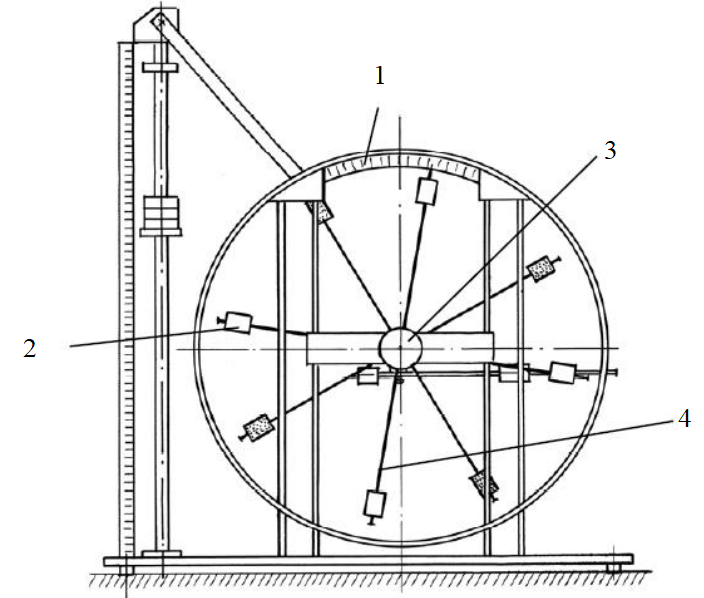
\includegraphics[width=0.5\textwidth]{pendulum.png}
\centering
\caption{Стенд лаборатории механики}
\end{figure}

1. Шкала
2. Груз
3. Рукоятка сцепления
4. Передняя крестовина

\item Метод экспериментального исследования:

Многократный прямой замер времени затухания колебаний и  их периода.

\item Рабочие формулы:

Период физического и математического маятника, их связь через приведённую длину:
\begin{equation}
T = 2\pi\sqrt{\frac{I}{mgl}}=2\pi\sqrt{\frac{l_\text{пр}}{g}}
\end{equation}

Связь логарифма отношения амплитуд с коэффициентом затухания:
\begin{equation}
\ln\frac{A}{A_0} = -\beta t
\end{equation}


Полный момент инерции:
\begin{equation} \label{eq:1}
I = I_0 + m_{\text{гр}}\left(R_{\text{верх.}}^2  + R_{\text{ниж.}}^2 + 2R_{\text{бок.}}^2\right)
\end{equation}

\item Измерительные приборы:

\begin{table}[H]
\centering
\begin{tabular}{|l|l|l|l|l|}
\hline
№ п/п & Наименование & Тип & Используемый диапазон & Погрешность прибора\\
\hline
1 & Секундомер смартфона & Электронный & 0 - 999.99 сек  & 0.01 сек\\
\hline
2 & Шкала & Ручной & $-30^\circ$ - $30^\circ$ & $1^\circ$\\
\hline
\end{tabular}
\end{table}

\item Параметры установки:

\begin{table}[H]
\centering
\begin{tabular}{|l|l|}
\hline
Параметр & Значение\\
\hline
Масса груза на крестовине & $408.0 \pm 0.5$г\\
\hline
Расстояние первой риски от оси & $57.0 \pm 0.5$мм\\
\hline
Расстояние между рисками & $25.0 \pm 0.2$мм\\
\hline
Высота груза на крестовине & $40.0 \pm 0.5$мм\\
\hline
\end{tabular}
\end{table}

\end{enumerate}
\section{Результаты измерений и их обработка}
\subsection{Прямые измерения}

Измерим время десяти ($N=10$) колебаний маятника при положении боковых грузов на 3-й риске и начальном отклонении в $30^{\circ}$:

\begin{table}[H]
\begin{center}
\begin{tabular}{|c|c|c|c|c|}
\hline
$t_1$, с & $t_1$, с & $t_3$, с & $t_{\text{ср}}$, с & $T$, с\\
\hline
17.93 & 17.80 & 17.98 & 17.90 & 1.79\\
\hline 
\end{tabular}
\caption{Результаты измерения времени 10 колебаний}
\end{center}
\end{table}

Измерим время, когда амплитуда отклонения маятника от равновесного положения будет равна $25^{\circ}$, $20^{\circ}$, 
$15^{\circ}$, $10^{\circ}$, $5^{\circ}$, при положении боковых грузов на 3-й риске и начальном отклонении в $30^{\circ}$:

\begin{table}[H]
\begin{center}
\begin{tabular}{|c|c|c|c|c|c|}
\hline 
\diagbox{Время}{Амплитуда откл.} & $25^\circ$ &  $20^\circ$ & $15^\circ$ & $10^\circ$ & $5^\circ$\\ 
\hline 
$t_1$, с & 37.47 & 87.33 & 142.36 & 209.50 & 311.79\\ 
\hline 
$t_2$, с & 43.19 & 87.64 & 137.17 & 200.88 & 301.37\\ 
\hline 
$t_3$, с & 48.70 & 98.66 & 150.23 & 219.46 & 311.31\\ 
\hline 
$t_{\text{ср}}$, с &43.12 & 91.21 & 143.25 & 209.95 & 308.16\\ 
\hline 
$\Delta {t}$, с &13.94 & 16.02 & 16.32 & 23.08 & 14.60\\ 
\hline 


\end{tabular}
\caption{Результаты измерений времени до достижения амплитуд отклонения.}
\label{tab:2}
\end{center}

\end{table}

Также измерим время десяти ($N=10$) колебаний маятника при различных расстояниях боковых грузов от центра (от 1-й до 6-й риски):


\begin{table}[H]
\begin{center}
\begin{tabular}{|c|c|c|c|c|c|c|}
\hline 
Число рисок & $t_1$, с & $t_2$, с  & $t_3$, с & $t_{\text{ср}}$, c  & $T$, с  & $\Delta T$, с\\ 
\hline 
$1$ & 16.19 & 16.07 & 16.06 & 16.1067  & 1.6107  & 0.0180 \\ 
\hline 
$2$ & 17.02 & 16.72 & 17.03 & 16.9233  & 1.6923  & 0.0437 \\ 
\hline 
$3$ & 18.02 & 18.12 & 18.00 & 18.0467  & 1.8047  & 0.0160 \\ 
\hline 
$4$ & 19.37 & 19.12 & 19.39 & 19.2933  & 1.9293  & 0.0374 \\ 
\hline 
$5$ & 20.73 & 20.52 & 20.63 & 20.6267  & 2.0627  & 0.0261 \\ 
\hline 
$6$ & 21.92 & 22.09 & 21.83 & 21.9467  & 2.1947  & 0.0328 \\ 
\hline 

\end{tabular}
\caption{Результаты измерений времени 10-ти колебаний при различных положениях боковых грузов.}
\label{tab:3}
\end{center}
\end{table}

\newpage
\subsection{Косвенные измерения и обработка результатов}
Используя результаты измерений зависимости амплитуды от времени, представленные в таблице \ref{tab:2}, построим график зависимости амплитуды колебаний от времени $A(t)$:

\begin{figure}[H]
\centering
\begin{tikzpicture}
\begin{axis}[
	axis lines = left,
	ylabel = \(A(t) \text{, град }(^\circ)\),
	xlabel = {\(t \text{, c}\)},
	ymin=0,	
	ymax=30,
	xmin=0,
	xmax=330,
	grid=both,
    grid style={line width=.1pt, draw=gray!10},
    major grid style={line width=.2pt,draw=gray!50},
    minor tick num=5,
	axis x line = bottom,
	axis line style ={line width = .3pt},
	legend style={at={(0.8, 0.8)},anchor=west}
	]


\addplot[blue1, mark size =2pt, mark=square*, error bars/.cd, y dir=both, y explicit, x dir=both, x explicit, error mark options={
      blue1,
      mark size=0.4pt,
      line width=4pt
    }, error bar style={fill=blue1,scale=2, line width=1pt}] table [y = DEV, y error = DEV_DIFF, x = TIME, x error = TIME_DIFF,  col sep=comma] {../ampl_dev_graph.csv};


\legend{$A(t)$}

\end{axis}
\end{tikzpicture}
\caption{График зависимости угловой амплитуды колебаний маятника $A$ от времени $t$.}
\label{gr:1}
\end{figure}

\subsubsection{Определение доминирующего типа трения}
Подробнее рассмотрим график \ref{gr:1}. Заметим, что амплитуда колебаний уменьшается не линейно, а по более сложной функции, напоминающей экспоненту (за каждые 50 секунд амплитуда уменьшается примерное в 1.25 раз). Такое затухание свойственно \textbf{вязкому трению}.



Для определения степени влияния вязкого трения на затухания колебаний аппроксимируем график $\ln{\frac{A}{A_0}} = -\beta t$ по МНК и найдём коэффициент затухания $\beta$:

\begin{figure}[H]
\centering
\begin{tikzpicture}
\begin{axis}[
	axis lines = left,
	ylabel = \(\ln{\frac{A}{A_0}}\),
	xlabel = {\(t \text{, c}\)},
	ymin=-2,	
	ymax=0,
	xmin=0,
	xmax=330,
	grid=both,
    grid style={line width=.1pt, draw=gray!10},
    major grid style={line width=.2pt,draw=gray!50},
    minor tick num=5,
	axis x line = bottom,
	axis line style ={line width = .3pt},
	legend style={at={(0.55, 0.85)},anchor=west}
	]


\addplot[only marks, blue3, mark size =2pt, mark=square*, error bars/.cd, y dir=both, y explicit, x dir=both, x explicit, error mark options={
      blue3,
      mark size=0.4pt,
      line width=4pt
    }, error bar style={fill=blue3,scale=2, line width=1pt}] table [y = LOG,  x = TIME, x error = TIME_DIFF,  col sep=comma] {../angle_coeff_graph.csv};
\addplot[blue1, domain=0:330] {-0.005460951996688503*x};

\legend{$\ln{\frac{A}{A_0}}$, Аппроксимация $-\beta*t$}

\end{axis}
\end{tikzpicture}
\caption{График зависимости логарифма отношения амплитуд от времени.}
\label{gr:2}
\end{figure}

При аппроксимации коэффициента затухания получаем:

\begin{equation*}
\beta \approx 0.00546 \pm 0.0004  \text{  сек}^{-1}
\end{equation*}

И время затухания:
\begin{equation*}
\tau = \frac{1}{\beta} \approx 183.12 \text{  сек}
\end{equation*}

Вычислим расстояния центров грузов от оси а также их их моменты инерции. К тому же, найдём полный момент инерции физического маятника $I$:


\begin{table}[H]
\begin{center}
\begin{tabular}{|c|c|c|c|c|c|c|}
\hline 
Риски & 1 &  2 & 3 & 4 & 5 & 6\\ 
\hline 
$R_\text{верх}$, мм & \multicolumn{6}{c|}{77.00}\\ 
\hline 
$\Delta R_\text{верх}$, мм & \multicolumn{6}{c|}{0.56}\\ 
\hline 
$R_\text{ниж}$, мм & \multicolumn{6}{c|}{202.00}\\ 
\hline 
$\Delta R_\text{ниж}$, мм & \multicolumn{6}{c|}{1.15}\\ 
\hline 
$R_\text{бок}$, мм & 77.00 & 102.00 & 127.00 & 152.00 & 177.00 & 202.00\\ 
\hline 
$\Delta R_\text{бок}$, мм & 0.56 & 0.59 & 0.69 & 0.82 & 0.98 & 1.15\\ 
\hline 
$I_\text{гр}$, $\text{кг}*\text{м}^2$ & 0.0239 & 0.0276 & 0.0322 & 0.0379 & 0.0446 & 0.0524\\ 
\hline 
$I$, $\text{кг}*\text{м}^2$ & 0.0319 & 0.0356 & 0.0402 & 0.0459 & 0.0526 & 0.0604\\ 
\hline 
$\Delta I$, $\text{кг}*\text{м}^2$ & 0.0002 & 0.0002 & 0.0002 & 0.0003 & 0.0003 & 0.0004\\ 
\hline 
$l_\text{пр эксп}$, мм & 643.99 & 710.95 & 808.46 & 924.02 & 1056.15 & 1195.65\\ 
\hline 
$l_\text{пр теор}$, мм & 625.03 & 696.56 & 788.08 & 899.58 & 1031.06 & 1182.53\\ 
\hline 



\end{tabular}
\caption{Приведённые длины и промежуточные значения.}
\label{tab:4}
\end{center}

\end{table}

Построим график $T^2(I)$ и, аппроксимируя его прямой по МНК, найдём произведение $ml$:


\begin{figure}[H]
\centering
\begin{tikzpicture}
\begin{axis}[
	axis lines = left,
	ylabel = \(T^2(I)\text{, c}^2\),
	xlabel = {\(I \text{, кг}*\text{м}^2 * 10^{-3}\)},
	ymin=1,	
	ymax=6,
	xmin=30,
	xmax=70,
	grid=both,
    grid style={line width=.1pt, draw=gray!10},
    major grid style={line width=.2pt,draw=gray!50},
    minor tick num=5,
	axis x line = bottom,
	axis line style ={line width = .3pt},
	legend style={at={(0.55, 0.35)},anchor=west}
	]


\addplot[only marks, blue4, mark size =2pt, mark=square*, error bars/.cd, y dir=both, y explicit, x dir=both, x explicit, error mark options={
      blue4,
      mark size=0.4pt,
      line width=4pt
    }, error bar style={fill=blue4,scale=2, line width=1pt}] table [y = PERIOD, y error = PERIOD_DIFF,  x = INERTIA, x error = INERTIA_DIFF,  col sep=comma] {../period_sqr_graph.csv};
\addplot[blue1, domain=30:70] {0.07891732831274925*x};

\legend{$T^2(I)$, Аппроксимация $4\pi^2\frac{I}{mgl}$}

\end{axis}
\end{tikzpicture}
\caption{График зависимости квадрата периода от момента инерции.}
\label{gr:3}
\end{figure}

Воспользовавшись МНК, получаем:
\begin{equation*}
\begin{aligned}
4\pi^2\frac{I}{mgl} &\approx  78.91\\
ml &\approx 0.051 \text{ кг*м} \\
  \end{aligned}
\end{equation*}

Предположив, что основная масса маятника сосредоточена в грузах на спицах, найдём из полученного значения $ml$ расстояние до оси вращения от цетра масс $l_{\text{теор.}}$:
\begin{equation*}
\begin{aligned}
l_{\text{теор.}} = \frac{ml}{4*m_\text{груз}} = 31.3 \text{ мм}
\end{aligned}
\end{equation*}

По периодам колебаний найдём экспериментальну приведённую длину $l_\text{пр.}$ и, используя расчитанное $l_{\text{теор.}}$, найдём $l_{\text{пр. теор.}}$. Внесём полученные значения в таблицу \ref{tab:4}.

\section{Вывод}
Таким образом, в ходе выполнения лабораторной работы удалось, измерив время затухания и периоды колебаний маятника при разлчных конфигурациях боковых грузов:
\begin{itemize}
\item[1.] Определить, что преобладающим типом трения в процессе затухании является - \textbf{вязкий тип трения} . 

На рисунке \ref{gr:1} легко видеть, что амплитуда колебаний затухает по экспоненциальному закону, что свойственно не сухому, а вязкому типу трения.

\item[2.] Проверить, что приведённая длина, полученная экспериментальынм путём, близка к приведённой длине теоретической. 

При этом с возрастанием расстояния боковых грузов от центра и, соответственно, возрастанием момента инерции маятника, приведённая длина увеличивается.

\end{itemize}


\section{Приложение}
Проект этой лабораторной работы, содержащий файлы с Python-кодом, использованным для вычислений и исходные TeX-файлы доступен по - \href{https://github.com/Dimankarp/Studies/tree/main/LaTeX/Physics%20-%20Damped%20Oscillations}{ссылке}.

\end{document}



